\documentclass[aps,prb,twocolumn,superscriptaddress,floatfix,longbibliography,10pt]{revtex4-2}

\usepackage[utf8]{inputenc}
\usepackage[spanish]{babel}
\usepackage{graphicx}
\usepackage{amsmath}
\usepackage{subcaption}
\usepackage{wrapfig} 
\usepackage[export]{adjustbox}

\usepackage{amsmath,amssymb} % math symbols
\usepackage{bm} % bold math font
\usepackage{graphicx} % for figures
\usepackage{comment} % allows block comments
\usepackage{textcomp} % This package is just to give the text quote '
%\usepackage{ulem} % allows strikeout text, e.g. \sout{text}

\usepackage[spanish]{babel}
% By dafault, spanish changes to a comma as decimal separator; to change to a dot, you can use \decimalpoint:
\decimalpoint

\usepackage{enumitem}
\setlist{noitemsep,leftmargin=*,topsep=0pt,parsep=0pt}

\usepackage{xcolor} % \textcolor{red}{text} will be red for notes
\definecolor{lightgray}{gray}{0.6}
\definecolor{medgray}{gray}{0.4}

%Para las tablas
\usepackage{multirow}

\usepackage{hyperref}
\hypersetup{
colorlinks=true,
urlcolor= blue,
citecolor=blue,
linkcolor= blue,
bookmarks=true,
bookmarksopen=false,
}

% Code to add paragraph numbers and titles
\newif\ifptitle
\newif\ifpnumber
\newcounter{para}
\newcommand\ptitle[1]{\par\refstepcounter{para}
{\ifpnumber{\noindent\textcolor{lightgray}{\textbf{\thepara}}\indent}\fi}
{\ifptitle{\textbf{[{#1}]}}\fi}}
\ptitletrue  % comment this line to hide paragraph titles
\pnumbertrue  % comment this line to hide paragraph numbers

% minimum font size for figures
\newcommand{\minfont}{6}

% Uncomment this line if you prefer your vectors to appear as bold letters.
% By default they will appear with arrows over them.
% \renewcommand{\vec}[1]{\bm{#1}}

%Cambiar Cuadros por Tablas y lista de...
%\renewcommand{\listtablename}{Índice de tablas}
\renewcommand{\tablename}{Tabla}
\renewcommand{\date}{Fecha}

%Para importar imágenes desde una carpeta:
\graphicspath{ {C:/Users/lupam/OneDrive/Escritorio/GitHub/Metodos_Num_Fluidos_I/Guias/Informe_final/Informe/Figures} {C:/Users/lupam/OneDrive/Escritorio/GitHub/Metodos_Num_Fluidos_I/Guias/Informe_final/Programa/graficos}}

\usepackage[bottom]{footmisc} %para que las notas al pie aparezcan en la misma página

\begin{comment}

%Comandos de interés:

* Para ordenar el documento:
\section{Introducción}
\section{\label{sec:Formatting}Formatting} %label para luego hacer referencia a esa sección

\ptitle{Start writing while you experiment} %pone nombre y título al documento dependiendo de si en el header están los comandos \ptitletrue y \pnumbertrue

* Ecuaciones:
\begin{equation}
a^2+b^2=c^2 \,.
\label{eqn:Pythagoras}
\end{equation}

* Conjunto de ecuaciones:
\begin{eqnarray}
\label{eqn:diagonal}
\nonumber d & = & \sqrt{a^2 + b^2 + c^2} \\
& = & \sqrt{3^2+4^2+12^2} = 13
\end{eqnarray}

* Para hacer items / enumerar:
\begin{enumerate}
  \item
\end{enumerate}

\begin{itemize}
  \item
\end{itemize}

* Figuras:
\begin{figure}[h]
    \includegraphics[clip=true,width=\columnwidth]{pixel-compare}
    \caption{}
     \label{fig:pixels}
\end{figure}

* Conjunto de figuras:
\begin{figure}
     \centering
     \begin{subfigure}[b]{0.3\textwidth}
         \centering
         \includegraphics[width=\textwidth]{graph1}
         \caption{$y=x$}
         \label{fig:y equals x}
     \end{subfigure}
     \hfill
     \begin{subfigure}[b]{0.3\textwidth}
         \centering
         \includegraphics[width=\textwidth]{graph2}
         \caption{$y=3sinx$}
         \label{fig:three sin x}
     \end{subfigure}
     \hfill
     \begin{subfigure}[b]{0.3\textwidth}
         \centering
         \includegraphics[width=\textwidth]{graph3}
         \caption{$y=5/x$}
         \label{fig:five over x}
     \end{subfigure}
        \caption{Three simple graphs}
        \label{fig:three graphs}
\end{figure}


* Para hacer referencias a fórmulas, tablas, secciones, ... dentro del documento:
\ref{tab:spacing}

* Para citar
Elementos de .bib
\cite{WhitesidesAdvMat2004}
url
\url{http://www.mendeley.com/}\\

* Agradecimientos:
\begin{acknowledgments}
We acknowledge advice from Jessie Zhang and Harry Pirie to produce Fig.\ \ref{fig:pixels}.
\end{acknowledgments}

* Apéndice:
\appendix
\section{\label{app:Mendeley}Mendeley}

* Bibliografía:
\bibliography{Hoffman-example-paper}

\end{comment}



\begin{document}

% Allows to rewrite the same title in the supplement
\newcommand{\mytitle}{\textcolor{red}{Título??}}

\title{\mytitle}

\author{Pablo Chehade \\
    \small \textit{pablo.chehade@ib.edu.ar} \\
    \small \textit{Métodos Numéricos en Fluidos I, Instituto Balseiro, CNEA-UNCuyo, Bariloche, Argentina, 2022} \\}


\begin{abstract}

\begin{itemize}
  \item Se estudiaron métodos numéricos espaciales y de evolución temporal para resolver el problema de la cavidad cuadrada hidrodinámica bidimensional.
  \item Se tiene en cuenta la ecuación de momentos y la de conservación de masa. Este tiene un término advectivo, uno difusivo.
  \item Se resolvió mediante el método de volumenes finitos y algoritmo simpler calculando presión y velocidades con grilla desplazada.
  \item En primer lugar, se estudió la dependencia de la solución en el estado estacionario con respecto al paso temporal.
  \item Se planteó un algoritmo para minimizar el costo computacional para encontrar el estado estacionario con un error menor al 5 \%
  \item En segundo lugar, se estudió el impacto en el estacionario del esquema espacial en el término advectivo empleando distintos números de Reynolds. En particular, se utilizaron diferencias centradas de orden 2, Up-wind de orden uno y el esquema QUICK de orden \textcolor{red}{?}
  \item Además, se estudió el orden de convergencia espacial de Up-wind de primer orden en referencia al mejor esquema advectivo
  \item Se evaluó el efecto de los pasos internos del algoritmo simpler
  \item Se estudió el efecto del método de evolución temporal, evaluando el estado transitorio de la solución mediante los métodos Euler Implícito y Crank-Nicholson
\end{itemize}


\end{abstract}

\maketitle

\textcolor{red}{Dudas:}
\begin{itemize}
  \item A mayor Re, mayor dt?
  \item $t_hat = tU_0/L$
\end{itemize}

\section{Introducción}

\ptitle{¿Por qué es importante resolver problemas de fluidos numéricamente? Rtas en la primera clase}

Gran parte de los problemas de mecánica de fluidos no son resolubles analíticamente. Algunos de ellos pueden ser estudiados experimentalmente, con el costo operativo y las dificultades para realizar las mediciones que esto conlleva \textcolor{red}{ref clase 1}. Una alternativa más rápida y de menor costo es resolverlos numéricamente. Si bien esto trae aparejado algunas dificultades, como los errores de aproximación numérica y el costo computacional, en los últimos años la resolución numérica de ecuaciones es aceptada y está ganando preponderancia.

\ptitle{Explicar el problema de la cavidad cuadrada hidrodinámica bidimensional}
Un problema muy estudiado desde el punto de vista numérico en mecánica de fluidos es el de la cavidad cuadrada hidrodinámica bidimensional, también conocido como Shear-drien cavity flow. En la figura \ref{fig:esquema_cavidad_cuadrada} se muestra un esquema del mismo. Consiste en una cavidad cuadrada bidimensional de lado $L$ que contiene un fluido incompresible de viscocidad $\nu$. Las condiciones de borde son de no deslizamiento en todas las paredes excepto en la horizontal superior. Sea $\vec{V}(x,y,t) = (u(x,y,t), v(x,y,t))$ la velocidad en el punto $(x,y)$ a tiempo $t$, las condiciones anteriores se traducen en $\vec{V}(x,0) = \vec{V}(0,y) = \vec{V}(L,y) = (0,0)$ y $\vec{V}(x,L) = (U_0(t),0)$.
\end{itemize}

\begin{figure}[h]
  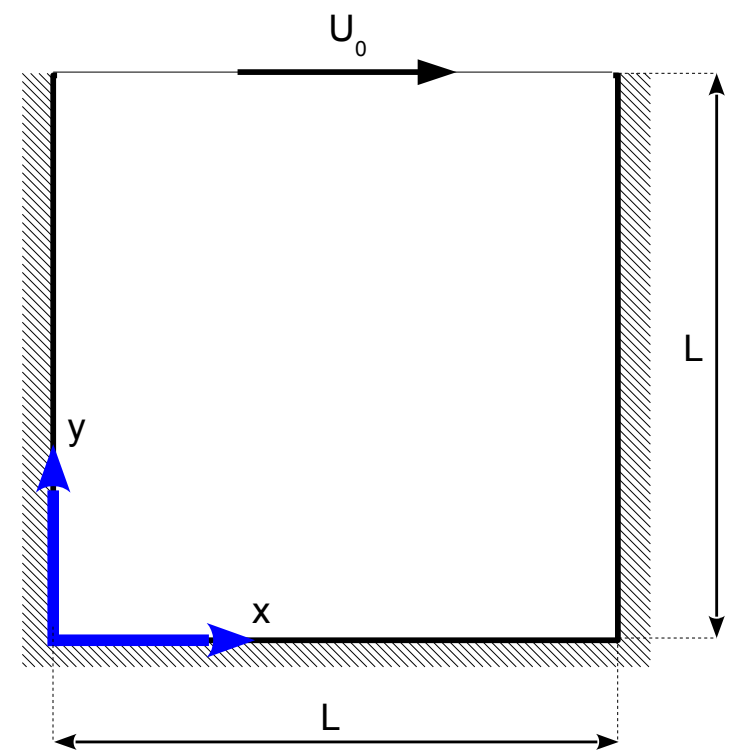
\includegraphics[clip=true,width=0.7\columnwidth]{esquema_cavidad_cuadrada.png}
  \caption{Esquema del problema de la cavidad cuadrada hidrodinámica bidimensional. Consiste en una cavidad cuadrada bidimensional de lado $L$ que contiene un fluido incompresible de viscocidad $\nu$. Las condiciones de borde son de no deslizamiento en todas las paredes excepto en la horizontal superior, con velocidad $U_0$. Esta figura fue extraída de \cite{Notas_materia}.}
   \label{fig:esquema_cavidad_cuadrada}
\end{figure}


\ptitle{Explicación de las ecuaciones involucradas}

El objetivo es determinar la presión $p(x,y,t)$ y las velocidades $u(x,y,t)$ y $v(x,y,t)$ para todo punto $(x,y)$ y tiempo $t$. Para esto se cuenta con tres ecuaciones diferenciales. En primer lugar, la ecuación de conservación de momento en las direcciones vertical y horizontal. Adimensionalmente, estas son
\begin{equation}
  \frac{\partial u}{\partial t} + \frac{\partial (u u)}{\partial x} + \frac{\partial (u v)}{\partial y} = - \frac{\partial p}{\partial x} + \frac{1}{Re} \left ( \frac{\partial^2 u}{\partial x^2} + \frac{\partial^2 u}{\partial y^2} \right ),
  \label{eq:momento_x}
\end{equation}
\begin{equation}
  \frac{\partial v}{\partial t} + \frac{\partial (u v)}{\partial x} + \frac{\partial (v v)}{\partial y} = - \frac{\partial p}{\partial y} + \frac{1}{Re} \left ( \frac{\partial^2 v}{\partial x^2} + \frac{\partial^2 v}{\partial y^2} \right ),
  \label{eq:momento_y}
\end{equation}
donde $Re = U_0L/\nu$ es el número de Reynolds. En ambas ecuaciones, el primer término del lado izquierdo resume la dependencia temporal del problema, los términos siguientes corresponden al efecto advectivo, el primer término del lado derecho resume la dependencia con la presión y los siguientes, el efecto difusivo. En segundo lugar se cuenta con la ecuación de conservación de masa. Para un fluido incompresible esta es
\[\bigtriangledown \bullet \vec{V} = \frac{\partial u}{\partial x} + \frac{\partial v}{\partial y} = 0.  \]
En base a esta ecuación se suele decir que el campo de velocidades tiene divergencia libre.

\ptitle{Resumen}

Empleando las tres ecuaciones diferenciales en derivadas parciales anteriores, es posible calcular la presión y las velocidades. Es notable que las soluciones dependerán del valor del número de Reynolds, el cual depende de la velocidad en la cara superior, la longitud de la cavidad y la viscocidad del líquido.

\section{Métodos Numéricos}

\ptitle{Resumen}
Para resolver el sistema de ecuaciones diferenciales es necesario discretizar el dominio y plantear esquemas numéricos para las ecuaciones diferenciales. En cuanto al primero, es necesario diferenciar entre dominio espacial y temporal. En cuanto al segundo, se emplearon volúmenes finitos con el objetivo de asegurar la conservación de masa \textcolor{red}{?} y se estudió el efecto de distintos métodos espaciales y temporales.

\subsection{Discretización del dominio}

\ptitle{Discretización espacial}
El dominio espacial se discretiza mediante una grilla uniforme con igual espaciamiento $\Delta$ en ambas direcciones. El número de volúmenes por dirección espacial es $n$ tal que $\Delta = 1/n$. En total se cuentan con $n^2$ volúmenes, cada uno numerado con los índices $i$ y $j$ para las direcciones horizontales y verticales, respecticamente. 

\ptitle{Grilla desplazada}
Se emplearon grillas desplazadas para las velocidades respecto a la presión. Estas se muestran esquemáticamente en la figura \ref{fig:grillas_desplazadas}. La grilla para $p$ posee todos sus volúmenes contenidos en la cavidad. Esto tiene la ventaja de no necesitar condiciones de borde sobre $p$, las cuales son difíciles de determinar, sino solo para $u$ y $v$.

\begin{figure}
  \centering
  \begin{subfigure}[b]{0.25\textwidth}
      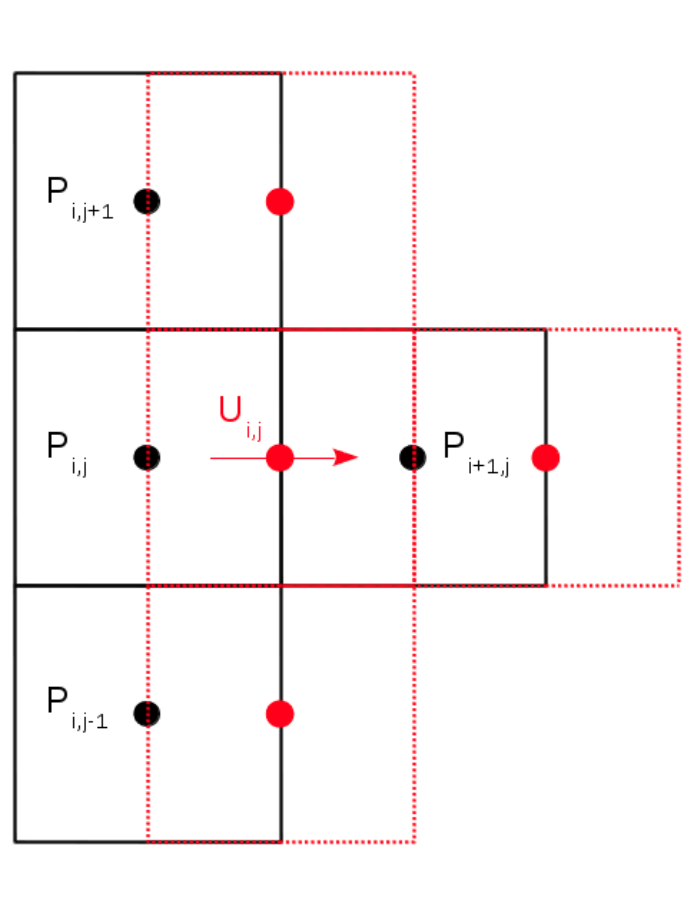
\includegraphics[width=\textwidth]{grilla_diferida_u.png}
      \caption{}
      \label{fig:grilla_desplazada_u}
  \end{subfigure}
  \hfill
  \begin{subfigure}[b]{0.2\textwidth}
      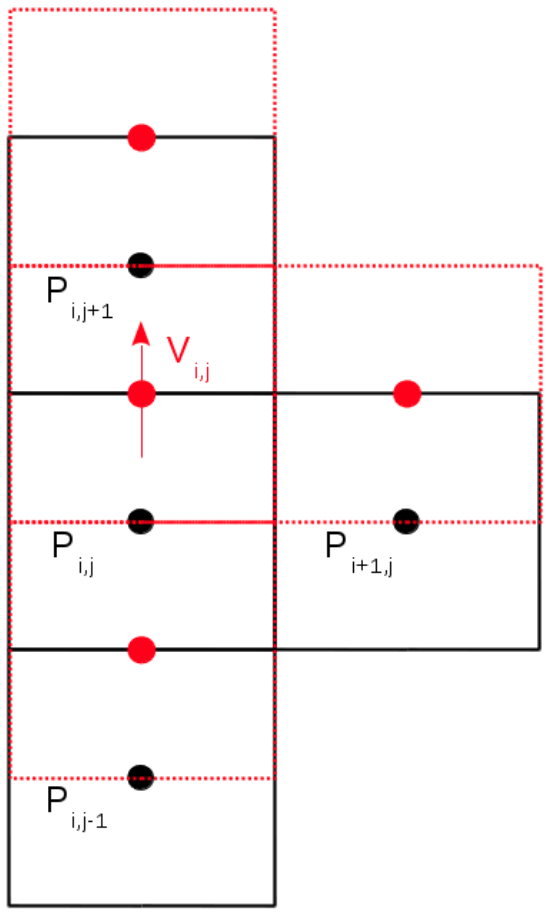
\includegraphics[width=\textwidth]{grilla_diferida_v}
      \caption{}
      \label{fig:grilla_desplazada_v}
  \end{subfigure}
     \caption{Esquema de las grillas desplazadas para la presión $p$ y las velocidades horizontal $u$ (\ref{fig:grilla_desplazada_u}) y vertical $v$ (\ref{fig:grilla_desplazada_v}). La grilla para $p$ es la única que posee todos sus volúmenes contenidos en la cavidad. Estas figuras fueron extraídas de \cite{Notas_materia}.}
     \label{fig:grillas_desplazadas}
\end{figure}


\ptitle{Discretización temporal}
Por otro lado, el dominio temporal se define desde $t = 0$ hasta $t = t_{max}$. De este modo, la variable temporal se discretizó en puntos equiespaciados $t_k = k \Delta t$ con $k = 0,1,\dots,M$ con $\Delta t = t_{max}/M$.

\subsection{Costo computacional}

\ptitle{Costo computacional y elección de $n$}
Debido a la cantidad de variables involucradas, proporcional a $n^2$, y dependiendo del número de pasos de tiempo a realizar, el costo computacional puede ser alto. En base a esto, es importante desarrollar métodos que permitan disminuir el costo pero que a su vez tengan una precisión aceptable. Un modo de minimizarlo es disminuyendo el número de variables pero exigiendo a su vez un error menor al 5 \%, por ejemplo. Sin embargo, para esto es necesario conocer la solución exacta o al menos una muy buena aproximación, lo cual no siempre se tiene.

\ptitle{Elección de $M$}
Otra alternativa es para dado $\Delta t$ elegir $M$ en base a un criterio de convergencia: si la solución tiende a un estacionario independiente del tiempo, entonces se avanza la solución hasta que, por ejemplo, se cumplan al mismo tiempos las desigualdades
\[\frac{du}{dt} < tol, \, \frac{dv}{dt} < tol \]
con $tol$ tolerancia. Claramente a menor $tol$, mayor el costo computacional debido a que se necesitan más pasos $M$. En este trabajo se decidió establecer $tol = 1 \times 10^{-5}$.

\ptitle{Elección de $\Delta t$}

Además, si solo es de interés la solución en el estado estacionario, otra alternativa es eligir $\Delta t$ de modo que la solución converja más rápido a pesar de tener un estado transitorio lejos de la solución exacta. Esto último se basa en la hipótesis de que la solución no depende del paso de tiempo, lo cual debe ser estudiado en detalle.

\ptitle{Resumen de costo computacional}
En este trabajo se estudiaron todos los métodos mencionados. En primer lugar, se determinó para $Re = 100$ y $1000$, el valor de $n_1$ tal que la solución numérica tiene un error menor al 5 \% respecto a una solución numérica de mayor precisión obtenida en \textcolor{red}{ref Guia}. En segundo lugar, estudiando la velocidad de convergencia en función de $\Delta t$ se planteó un algoritmo que permita elegir $\Delta t$ de modo de minimizar el número de pasos de tiempo necesarios. En tercer lugar, se decidió emplear el criterio de elección de $M$ durante todo el trabajo.



\subsection{Esquema numérico}

\ptitle{Resumen}
\begin{itemize}
  \item Se construyó un esquema numérico del sistema de ecuaciones \textcolor{red}{REFs}.
  \item Se empleó volúmenes finitos para asegurar la conservación de la masa.
  \item Se emplearon distintos métodos numéricos y se analizó su efecto en la solución numérica
  \item Para la evolución temporal se empleó Euler Implícito y Crank-Nicolson
  \item En cuanto a la discretización espacial, para el término advectivo se empleó DC2, UP1 y QUICK. Para el de presión, \textcolor{red}{cuál?} y para el difusivo, DC2-
  \item Una vez planteado el esquema numérico, se resolvió el sistema de ecuaciones mediante el algoritmo SIMPLER. A continuación se explica brevemente cada método numérico utilizado y las ventajas o desventajas que trae aparejado su utilización.
\end{itemize}

\ptitle{Volúmenes finitos}
\begin{itemize}
\item La implementación del esquema de volúmenes finitos se explica en detalle en \cite{Notas_materia}.
\item Se integran las ecuaciones de momento \ref{eq:momento_x} y \ref{eq:momento_y} en el volumen de las grillas de $u$ y $v$, respecticamente, empleando la regla del rectángulo \textcolor{red}{ref Moin}. Esta aproximación es de orden mayor a $\Delta^2$, correspondiente al mayor orden de aproximación de los esquemas espaciales.Se llega a un sistema de ecuaciones donde
\item El término temporal depende de $du_{ij}/dt$
\item El término advectivo depende de $u$ evaluado en los cuatro laterales: ($u_{n,ij}$ norte, $y$). Idéntico para $v$
\item El término de presión depende de $p_{ij}$
\item El término difusivo depende de las derivadas espaciales de $u$ evaluadas en los laterales:
\item La aplicación de determinado método numérico es aproximar esos valores
\item una particularidad del término advectivo es que en su integral, por ejemplo
\[ \]
aparecen términos no lineales. Uno de ellos se calculará usando el del paso anterior para evitar la no linealidad.
\end{itemize}



\ptitle{Método de evolución temporal}
El sistema de ecuaciones anterior se puede llevar mediante un cambio de variables a un sistema de ecuaciones del tipo
\[ \]
donde y vec
El método de Euler Implícito se basa En

El método de Crank-Nicholson

COPIAR DEL INFORME 2

\ptitle{Métodos para el término advectivo}
\begin{itemize}
  \item En base al desarrollo presentado en \cite{Notas_materia}, para discretizar el sistema de ecuaciones diferenciales, basta con especificar un método para aproximar $U_w$, $V_s$, \dots
\end{itemize}



\ptitle{Algoritmo simpler simplificadamente}
\begin{itemize}
  \item \cite{Patankar}
  \item Es un algoritmo segregado o de paso fraccionado. Esto último en el sentido de que se calculan por separado $\vec{v}$ y $p$.
  \item Permite calcular la velocidad con divergencia libre (cumple la conservación de masa) y la presión en cada paso de tiempo a partir de un guess, el cual suele ser la solución del paso anterior. \textcolor{red}{es así, no?}
  \item Se propone que determinados términos de la ecuación se pueden estimar con el paso anterior. Se calcula la presión de modo de que el nuevo campo de velocidades tenga divergencia libre. Luego se calcula el campo de velocidades empleando esta nueva presión, obteniendo un campo que no necesariamente tiene divergencia libre. Posteriormente, se vuelve a calcular la presión de modo que el nuevo campo de velocidades tenga divergencia libre, empleando como guess el campo de velocidades calculado. Este proceso es un paso del algoritmo simpler.
  \item En el link \url{https://www.cfd-online.com/Wiki/SIMPLER_algorithm_-_SIMPLE_-_Revised} se explica el procedimiento bien resumido y sin ecuaciones.
  \item La exactitud de la solución depende del número de pasos internos realizados en el algoritmo, que pueden ser tantos como uno quiera aunque aumenta el costo computacional
\end{itemize}



\textcolor{red}{Es necesario explicar cómo discretizar las ecuaciones de momento? Sería copiar textual el desarrollo hecho en la penúltima clase. Le pregunté a Federico}
\textcolor{red}{Plantear lo siguiente luego de que Federico me halla respondido}

\ptitle{Esquemas numéricos posibles para cada término}
\begin{itemize}
  \item Para cada término de las ecuaciones de momento, se pueden plantear distintos esquemas numéricos. En este trabajo se estudiaron los siguientes:
  \begin{itemize}
    \item Para la parte temporal, se emplearon los esquemas de Euler implícito y de Crank-Nicolson.
  \end{itemize}
\end{itemize}

\ptitle{Término advectivo. Explicar cada método numérico}
\begin{itemize}
  \item 
\end{itemize}

\ptitle{Término temporal. Explicar cada método numérico}
\begin{itemize}
  \item 
\end{itemize}



\ptitle{Resumen de lo que se va a estudiar}
\begin{itemize}
  \item En primer lugar, se estudió la dependencia de la solución en el estado estacionario con respecto al paso temporal.
  \item Se planteó un algoritmo para minimizar el costo computacional para encontrar el estado estacionario con un error menor al 5 \%
  \item Se evaluó el efecto de los pasos internos del algoritmo simpler
  \item En segundo lugar, se estudió el impacto en el estacionario del esquema espacial en el término advectivo empleando distintos números de Reynolds. En particular, se utilizaron diferencias centradas de orden 2, Up-wind de orden uno y el esquema QUICK de orden \textcolor{red}{?}
  \item Además, se estudió el orden de convergencia espacial de Up-wind de primer orden en referencia al mejor esquema advectivo
  \item Se estudió el efecto del método de evolución temporal, evaluando el estado transitorio de la solución mediante los métodos Euler Implícito y Crank-Nicholson
\end{itemize}





\begin{itemize}
  \item \textcolor{red}{En todos los casos se usó una tolerancia para el estado estacionario de 1e-5}
\end{itemize}

\section{Resultados y discusión}


\subsection{Dependencia del estado estacionario con el paso dt}

En primer lugar, se analizó la dependencia del estado estacionario con el paso de evolución temporal. Se calculó $u(0.5,0.5)$ y $v(0.5,0.5)$ para $Re = 1000$, $n_1 = 20$ y distintos $\Delta t$ entre $0.005$ y $20$. Se emplearon diferencias centradas de orden 2 para el término advectivo y Euler implícito para la evolución temporal. En la figura \ref{fig:a_vel_vs_dt} se grafican los resultados obtenidos respecto al valor correspondiente al menor $\Delta t$ en valor absoluto. Se observa una diferencia entre los valores obtenidos del orden de $1 \times 10^{-4}$, ligeramente superior a la tolerancia en el criterio de convergencia. Aunque si solo se consideraran $\Delta t$ menores a 1, se obtendría una diferencia menor a dicha tolerancia.

Esto indica que el estado estacionario depende de $\Delta t$ con una variación menor a la tolerancia siempre que ocurra $\Delta t < 1$ \textcolor{red}{menor pero del orden}. Si bien esto sólo se da en el caso particular considerado, se tomará como normal general



\begin{figure}[h]
  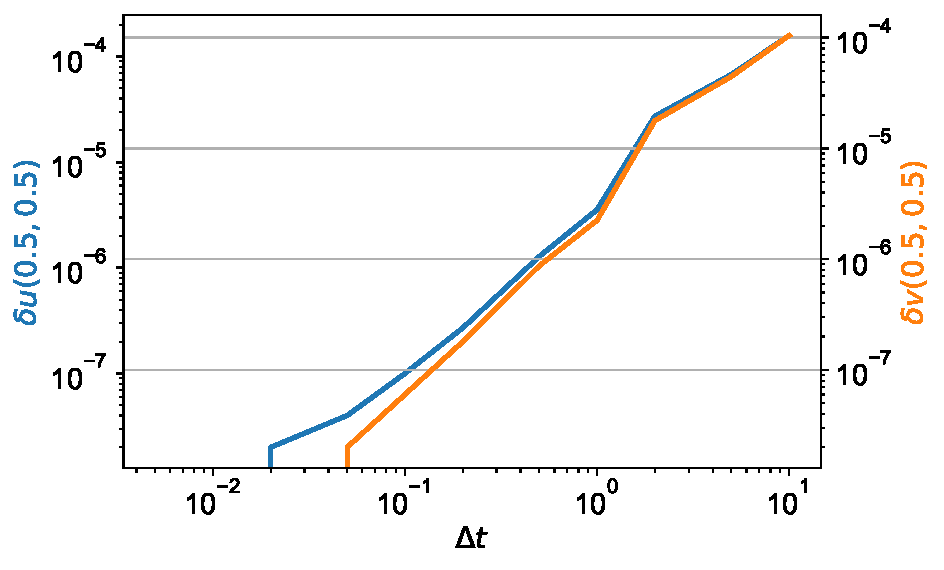
\includegraphics[clip=true,width=\columnwidth]{a_vel_vs_dt.pdf}
  \caption{}
   \label{fig:a_vel_vs_dt}
\end{figure}



\subsection{Elección de dt}

\begin{itemize}
  \item Como se mencionó en la sección anterior, debido a la cantidad de variables involucradas el costo computacional necesario para encontrar el estado estacionario es muy alto.
  \item Además, el resultado anterior indica que el estado estacionario podría no depender del paso de tiempo $\Delta t$.
  \item Por lo tanto, si solo es de interés el estado estacionario, se puede elegir $\Delta t$ de modo que el número de pasos necesarios sea el menor posible.
  \item Esto no implica necesariamente que $\Delta t$ sea lo mayor posible.
  \item En base a esto, se propone el siguiente algoritmo.
\end{itemize}

\ptitle{Algoritmo}
\begin{itemize}
  \item 
\end{itemize}

\ptitle{Para qué se usó el algoritmo anterior}
\begin{itemize}
  \item Este algoritmo no siempre va a encontrar el mejor $\Delta t$ posible, pero se espera que esté cerca del óptimo.
  \item El algoritmo anterior fue empleado para hallar el estado estacionario en todo este trabajo salvo el caso particular $n_1 = 80$. Este es el caso más costoso y se buscará a mano el mejor $\Delta t$ para cada $Re$ específico.
  \item Se usaron $\Delta t = 0.35$, $1.25$ y $2.0$ para $Re = 100$, $1000$ y $5000$, respecticamente
\end{itemize}

\subsection{dt para distintos lsimpler}

Estaría bueno dar para cada caso el máximo dt posible y el que me da mi algoritmo

\subsection{Término advectivo}
\textcolor{red}{Los captions no están siendo autocontenidos. Hay que mencionar qué curva se encima sobre cuál}


Se implementó para el término advectivo los esquemas DC2, UP1 y QUICK. Se calculó el estado estacionario para $Re = 100, 1000 \, \mathrm{y} \, 5000$, para $n1 = 20, 40 \, \mathrm{y} \, 80$ y para los tres esquemas mencionados

Es de interés estudiar
\begin{itemize}
  \item La dependencia con el número de Reynolds
  \item La dependencia con n1
  \item La dependencia con el termino advectivo
\end{itemize}

\ptitle{Comparación DC2 vs n1 para distintos Re}
En primer lugar, se estudió la dependencia del estado estacionario con la discretización espacial $n_1$ y el número de $Re$, empleando como término advectivo particular diferencias finitas de orden 2
\begin{itemize}
  \item En las figuras \ref{fig:velocidades_u_DC2_vs_Re} y \ref{fig:velocidades_v_DC2_vs_Re} se grafican las velocidades $u(0.5,y)$ y $v(x,0.5)$ para distintos casos.
  \item Para $Re = 100$ se observa en ambos casos que el resultado varía cualitativamente poco con el tamño de la discretización.
  \item Por otro lado, para $Re = 1000$ la diferencia entre los resultados es más significativa, llegando en algunos sitios a superar la tolerancia de $1 \times 10^{-5}$ del criterio de convergencia.
  \item Por último, el caso $Re = 5000$ es el más notable de todos. Ni siquiera la solución de mayor $n_1$ es cercana a la de referencia
  \item Esto indica que a mayor número de $Re$ es necesario disminuir el tamaño de la discretización, es decir, aumentar $n_1$, para obtener una solución más precisa.
  \item \textcolor{red}{Por qué pasa esto? Qué tiene de particular el caso de $Re$ alto?}
\end{itemize}

\ptitle{Comparación cualitativa entre métodos numéricos para distintos Re}
En segundo lugar, se estudió la dependencia del estado estacionario con el número de $Re$ y el método numérico empleado para el término advectivo. En todos los casos se empleó $n_1 = 80$

\begin{itemize}
  \item En las figuras \ref{terminos_advs_u} y \ref{terminos_advs_u} se grafica
  \item Cualitativamente, para $Re = 100$ no se observan grandes diferencias.
  \item Para $Re = 1000$ es notable que el método UP1 no aproxima correctamente la solución, mientras que DC2 y QUICK sí lo hacen. Esto se puede justificar en los órdenes de aproximación de los métodos, siendo el primero de orden 1 y los segundos de orden 2 \textcolor{red}{QUICK es orden 2?}
  \item Para $Re = 5000$ ninguno de los métodos aproxima correctamente la solución en la totalidad del dominio. En base a los resultados obtenidos al variar $n_1$, esto podría deberse al tamaño de la grilla espacial y no al método numérico.
\end{itemize}

\ptitle{Comparación numérica entre métodos numéricos para distintos $Re$.}
Para cada variación posible de $n_1$, $Re$ y método para el término advectivo, se calculó el error relativo $e_{rel}$ respecto a la bibliografía \textcolor{red}{referencia} en el centro del dominio $x = 0.5$ e $y = 0.5$. Para calcular este error se suman cuadráticamente los errores en $u$ y $v$ y se normaliza con el valor de referencia, es decir,
\[e_{rel} = \frac{\sqrt{(u_{exp} - u_{sol})^2 + (v_{exp} - v_{sol})^2}}{\sqrt{u_{sol}^2 + v_{sol}^2}}. \]

Mencionar cómo se calcula $u(0.5,0.5)$ y que sólo tiene sentido calcularlo allí porque la aproximación es del mismo orden que los métodos. Calcularla en otro lado con un promedio ponderado es de mayor orden.

\begin{itemize}
  \item En la figura \ref{fig:termino_advectivo}. Esta permite hacer una discusión cualitativa
  \item Cualitativamente los tres métodos muestran el mismo comportamiento
  \item En primer lugar, independientemente del valor de $Re$, a mayor $n_1$, menor error. La excepción a este caso es el de $Re = 100$ y $n_1 = 80$, donde tanto en DC2 como en QUICK no se cumple la regla \textcolor{red}{por qué será?}
  \item En segundo lugar, a mayor $Re$, el error tiende a aumentar. Esto se observó en los análisis anteriores: a mayor $Re$ es necesario aumentar $n_1$ para obtener una solución más precisa.
  \item Para comparar los métodos numéricos entre sí, es necesario analizar cuantitativamente los errores.
  \item Estos se presentan para $n_1 = 80$ CREO en la TABLA REF. Tengo que cambiar la tabla, tiene que decir los nros de Re en lugar de $e$
  \item Se observa que el método DC2 presenta menor error.
\end{itemize}

$tol_estacionario = 1e-5$

\begin{itemize}
  \item En la figura \ref{velocidades_DC2_vs_Re}
\end{itemize}


\onecolumngrid


\begin{figure}
  \centering
  \begin{subfigure}[b]{0.32\textwidth}
      \centering
      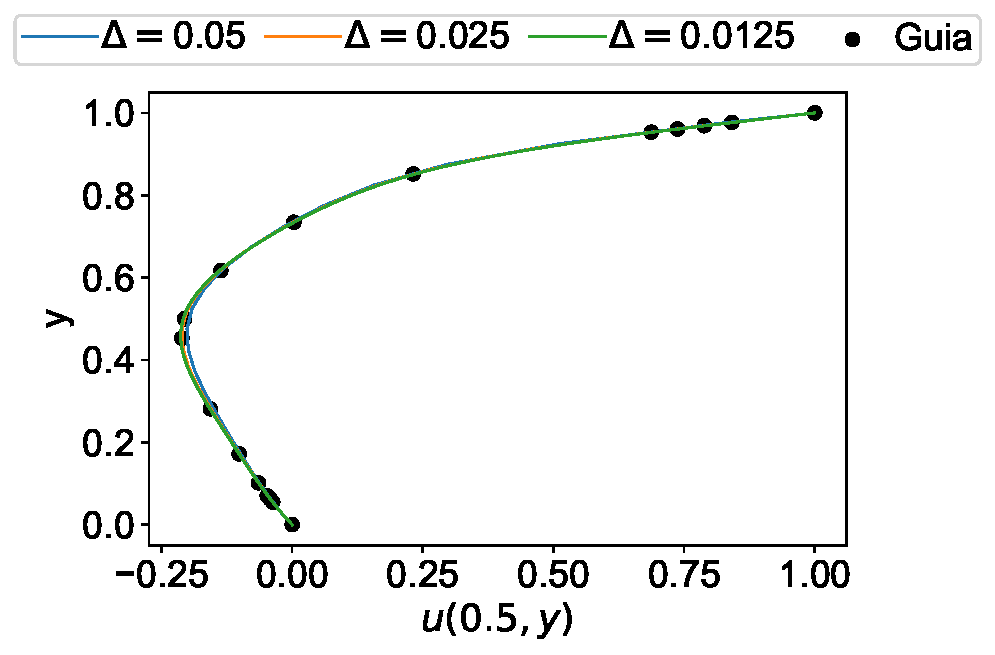
\includegraphics[width=\textwidth]{termino_adv_Db_u_100.pdf}
      \caption{}
      \label{fig:termino_adv_Db_u_100}
  \end{subfigure}
  \hfill
  \begin{subfigure}[b]{0.32\textwidth}
      \centering
      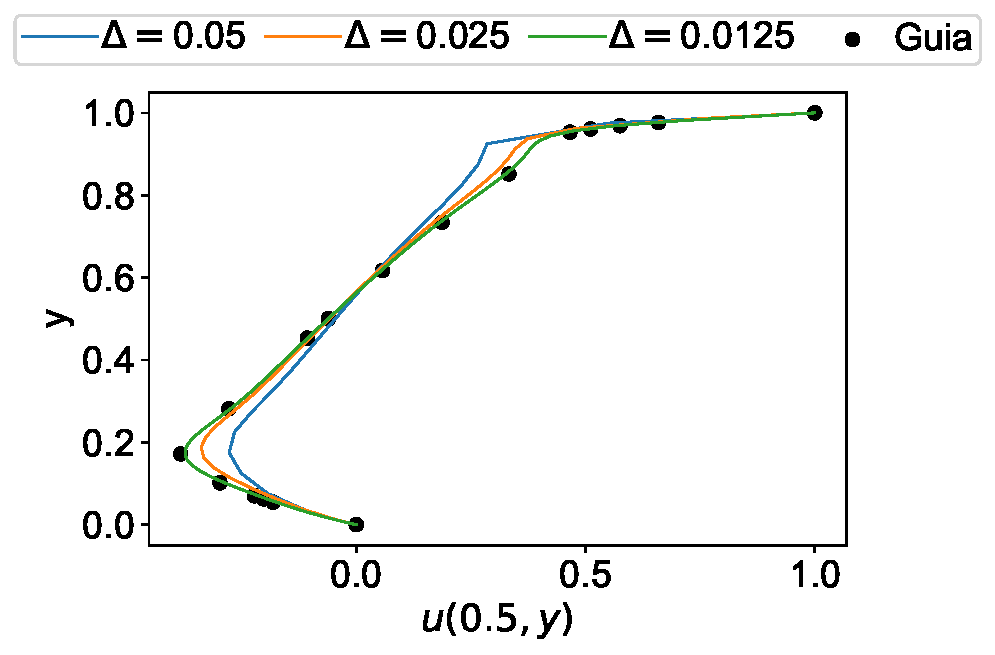
\includegraphics[width=\textwidth]{termino_adv_Db_u_1000.pdf}
      \caption{}
      \label{fig:termino_adv_Db_u_1000}
  \end{subfigure}
  \hfill
  \begin{subfigure}[b]{0.32\textwidth}
      \centering
      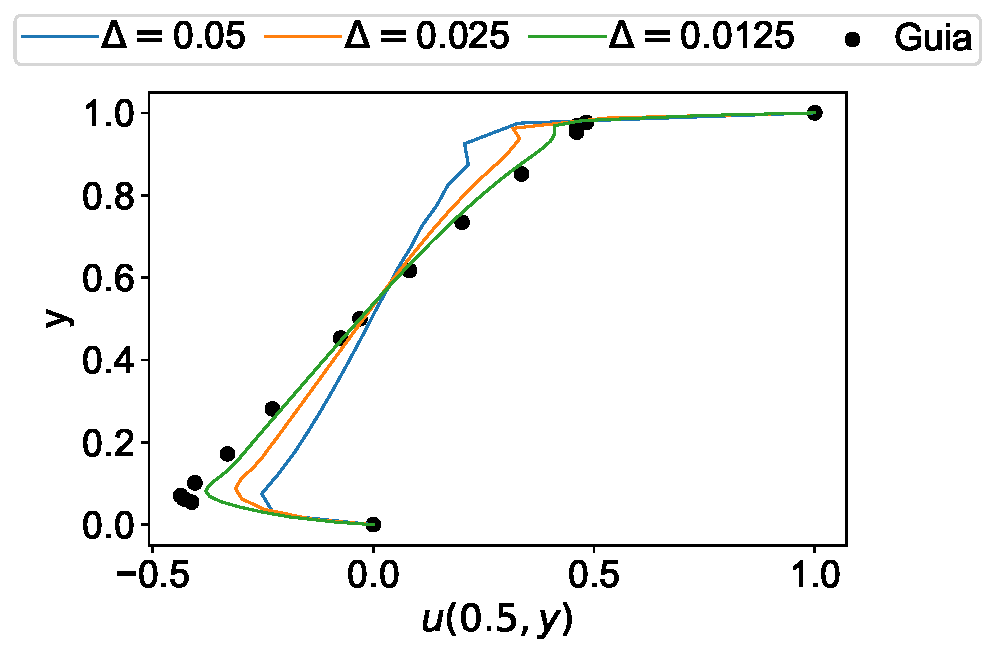
\includegraphics[width=\textwidth]{termino_adv_Db_u_5000.pdf}
      \caption{}
      \label{fig:termino_adv_Db_u_5000}
  \end{subfigure}
     \caption{Velocidad $u(0.5,y)$ en función de $y$ para distinto tamaño de la grilla espacial $n_1$ y número de Reynolds $Re$: (a) $Re = 100$, (b) $Re = 1000$ y (c) $Re = 5000$.}
     \label{fig:velocidades_u_DC2_vs_Re}
\end{figure}

\begin{figure}
  \centering
  
  \begin{subfigure}[b]{0.32\textwidth}
    \centering
    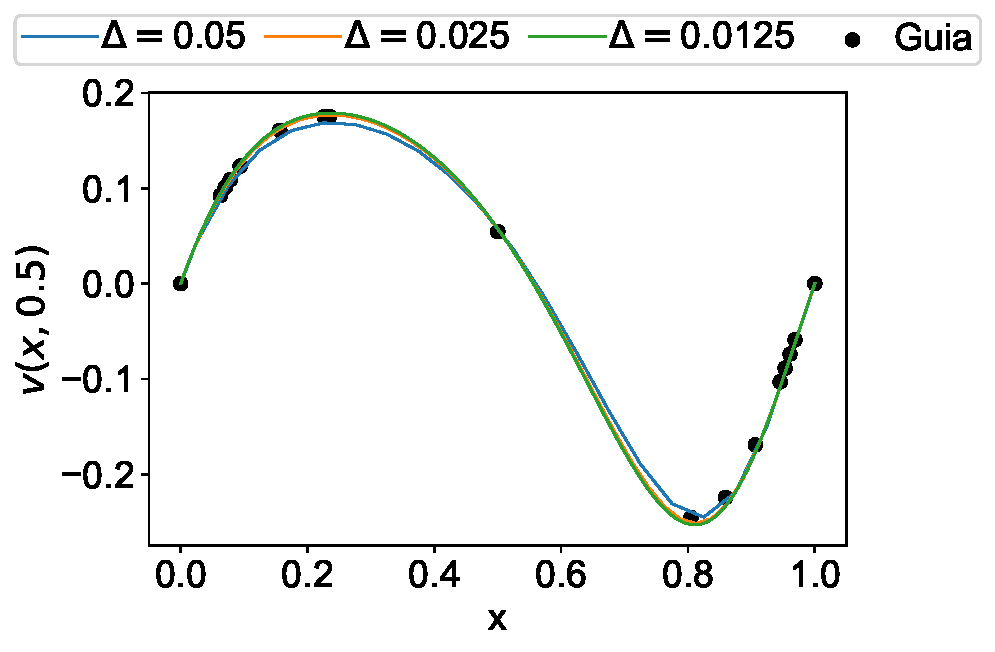
\includegraphics[width=\textwidth]{termino_adv_Db_v_100.pdf}
    \caption{}
    \label{fig:termino_adv_Db_v_100}
\end{subfigure}
\hfill
\begin{subfigure}[b]{0.32\textwidth}
    \centering
    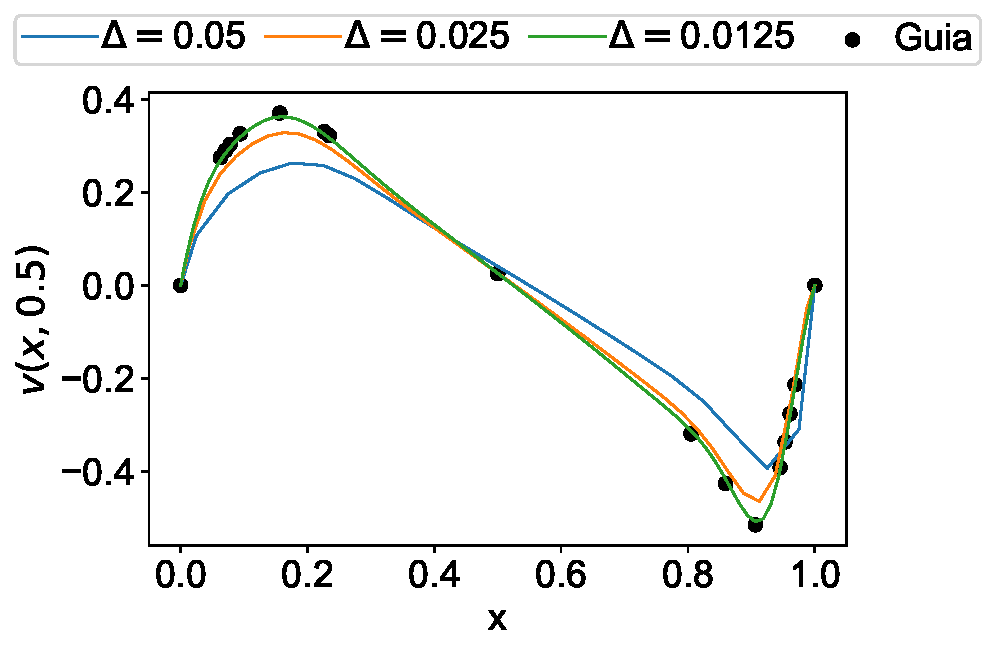
\includegraphics[width=\textwidth]{termino_adv_Db_v_1000.pdf}
    \caption{}
    \label{fig:termino_adv_Db_v_1000}
\end{subfigure}
\hfill
\begin{subfigure}[b]{0.32\textwidth}
    \centering
    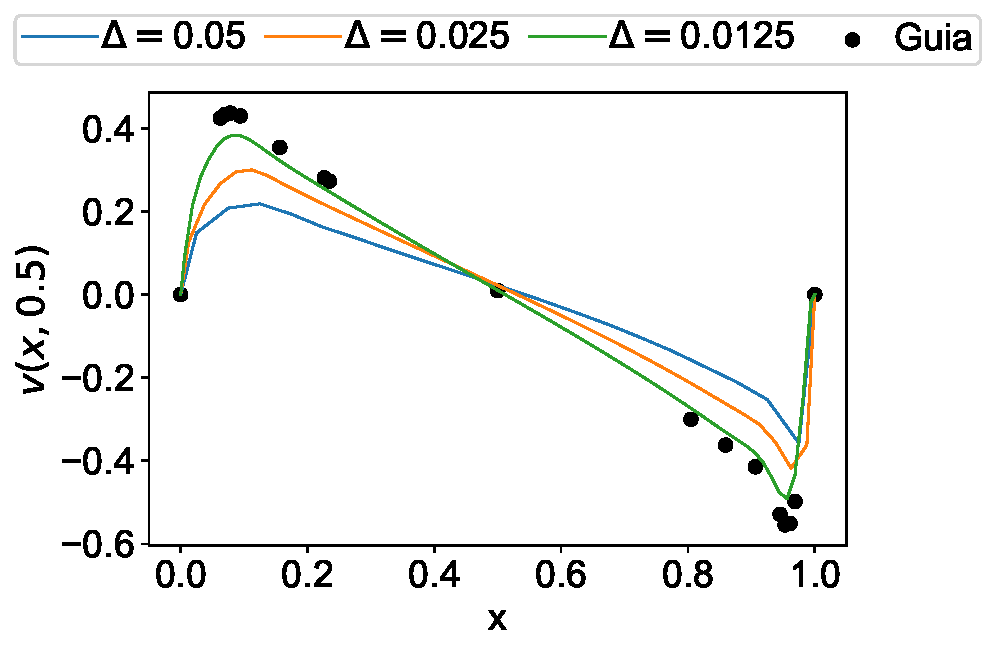
\includegraphics[width=\textwidth]{termino_adv_Db_v_5000.pdf}
    \caption{}
    \label{fig:termino_adv_Db_v_5000}
\end{subfigure}
     \caption{Velocidad $v(x,0.5)$ en función de $x$ para distintos tamaño de la grilla espacial $n_1$ y número de Reynolds $Re$: (d) $Re = 100$, (e) $Re = 1000$ y (f) $Re = 5000$.}
     \label{fig:velocidades_v_DC2_vs_Re}
\end{figure}





\begin{figure}
  \centering
  \begin{subfigure}[b]{0.32\textwidth}
      \centering
      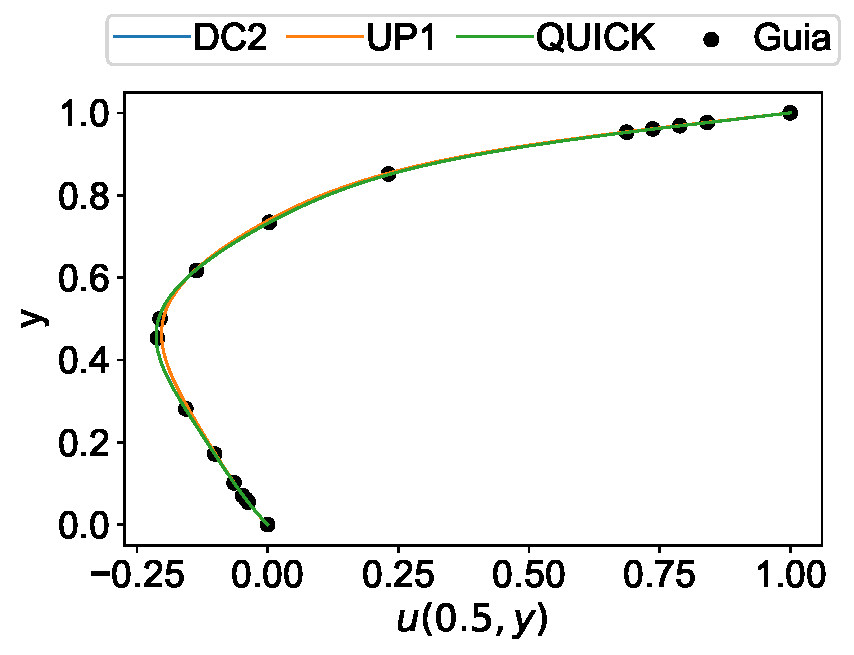
\includegraphics[width=\textwidth]{terminos_advs_u_100.pdf}
      \caption{}
      \label{fig:terminos_advs_u_100}
  \end{subfigure}
  \hfill
  \begin{subfigure}[b]{0.32\textwidth}
      \centering
      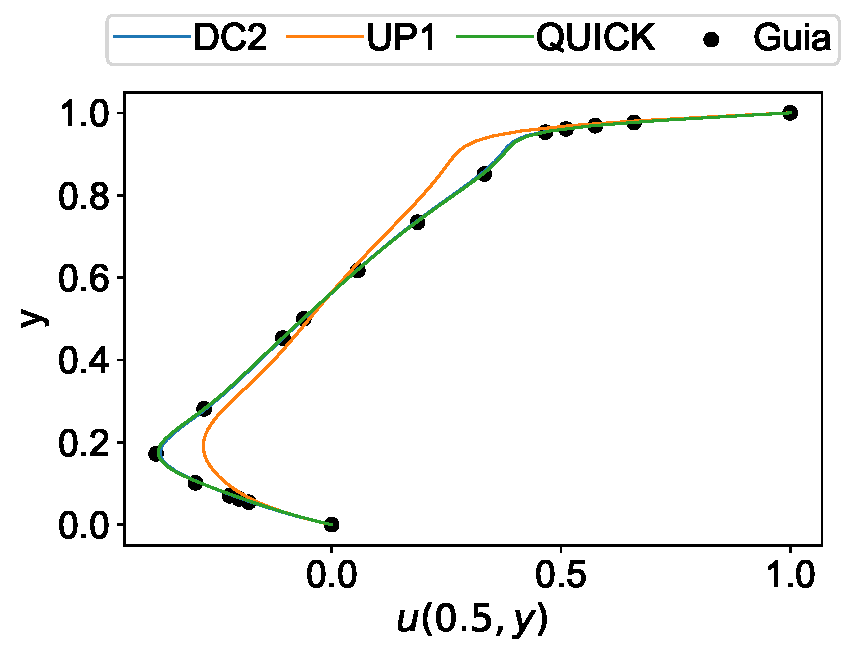
\includegraphics[width=\textwidth]{terminos_advs_u_1000.pdf}
      \caption{}
      \label{fig:terminos_advs_u_1000}
  \end{subfigure}
  \hfill
  \begin{subfigure}[b]{0.32\textwidth}
      \centering
      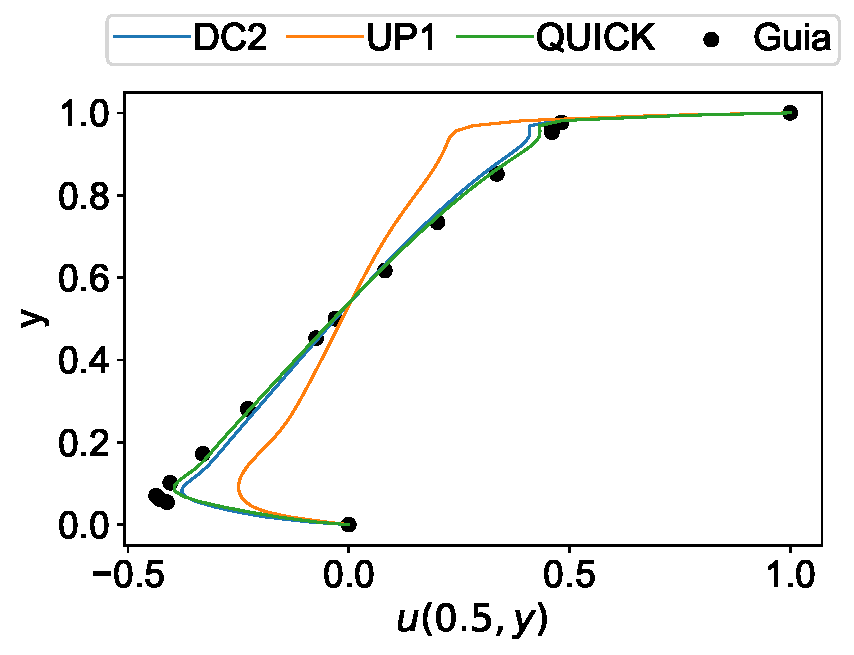
\includegraphics[width=\textwidth]{terminos_advs_u_5000.pdf}
      \caption{}
      \label{fig:terminos_advs_u_5000}
  \end{subfigure}
     \caption{Velocidad $u(0.5,y)$ en el estado estacionario en función de $y$ para distintas métodos numéricos del término advectivo y distintos números de $Re$: (a) $Re = 100$, (b) $Re = 1000$ y (c) $Re = 5000$. En todos los casos se empleó una grilla espacial de tamaño $n_1 \times n_1$ con $n_1 = 80$}
     \label{fig:terminos_advs_u}
\end{figure}

\begin{figure}
  \centering
  \begin{subfigure}[b]{0.32\textwidth}
    \centering
    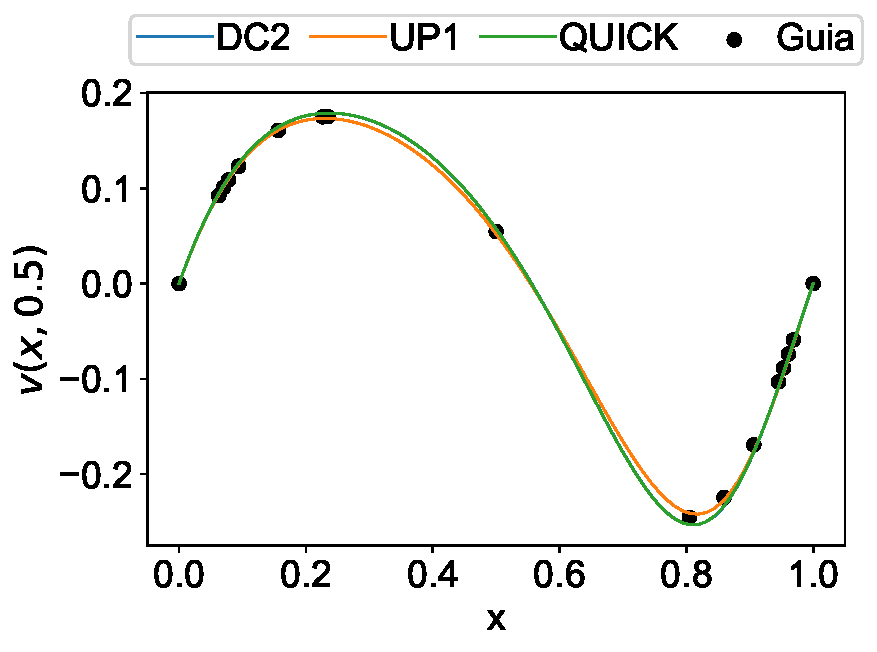
\includegraphics[width=\textwidth]{terminos_advs_v_100.pdf}
    \caption{}
    \label{fig:terminos_advs_v_100}
  \end{subfigure}
  \hfill
  \begin{subfigure}[b]{0.32\textwidth}
    \centering
    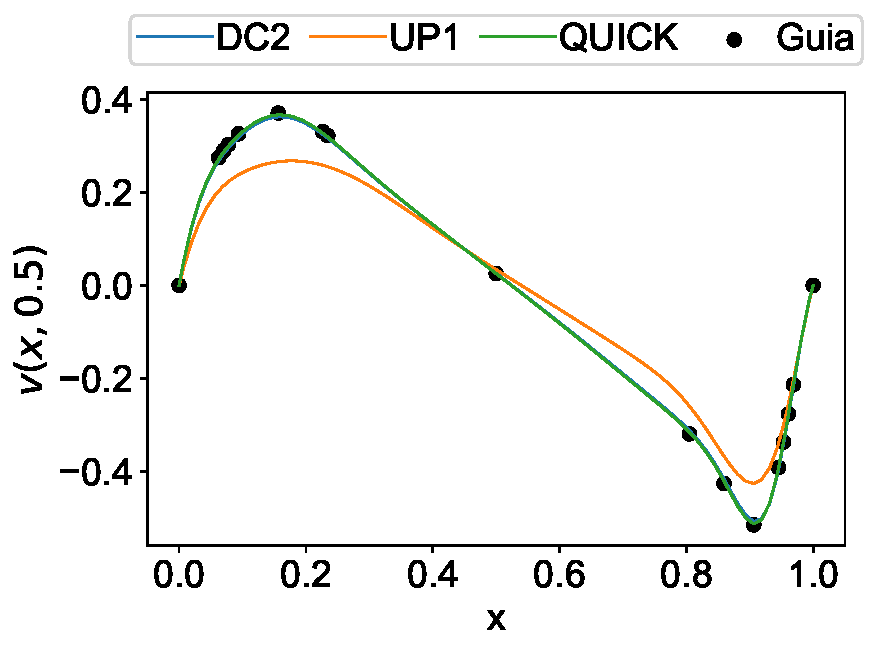
\includegraphics[width=\textwidth]{terminos_advs_v_1000.pdf}
    \caption{}
    \label{fig:terminos_advs_v_1000}
  \end{subfigure}
  \hfill
  \begin{subfigure}[b]{0.32\textwidth}
    \centering
    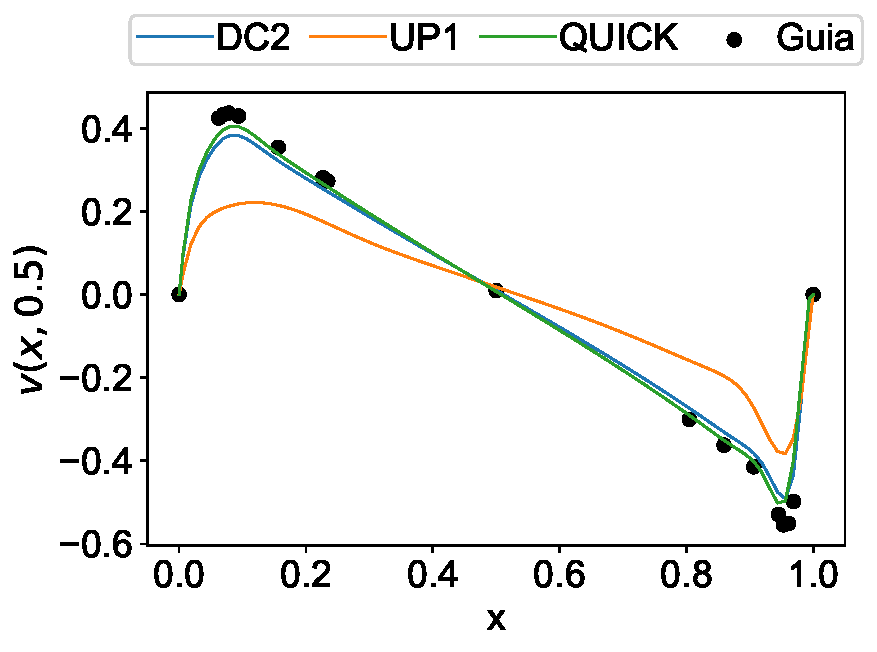
\includegraphics[width=\textwidth]{terminos_advs_v_5000.pdf}
    \caption{}
    \label{fig:terminos_advs_v_5000}
  \end{subfigure}
     \caption{}
     \label{fig:terminos_advs_v}
\end{figure}




\begin{figure}
  \centering
  \begin{subfigure}[b]{0.32\textwidth}
      \centering
      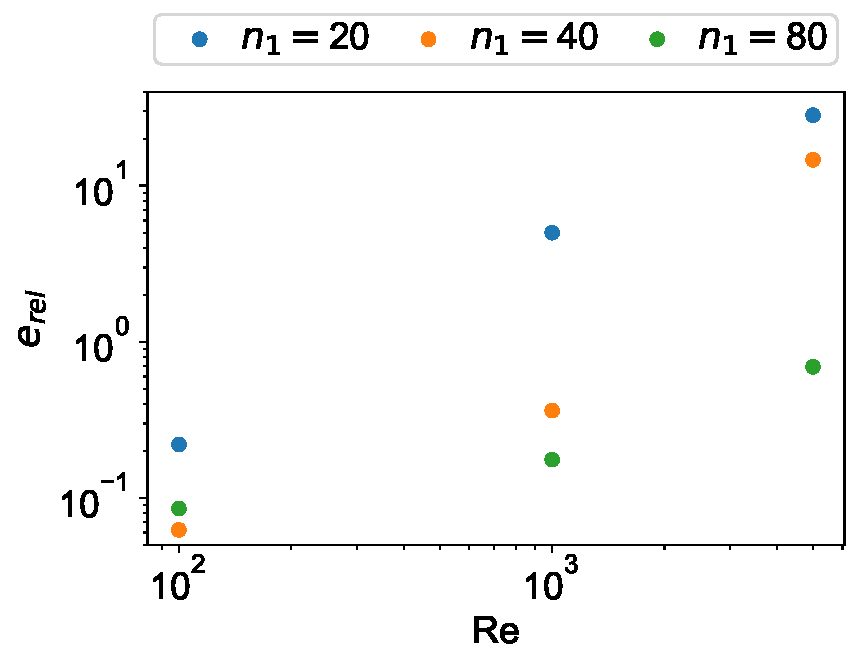
\includegraphics[width=\textwidth]{termino_adv_DC2.pdf}
      \caption{}
      \label{fig:termino_adv_DC2}
  \end{subfigure}
  \hfill
  \begin{subfigure}[b]{0.32\textwidth}
      \centering
      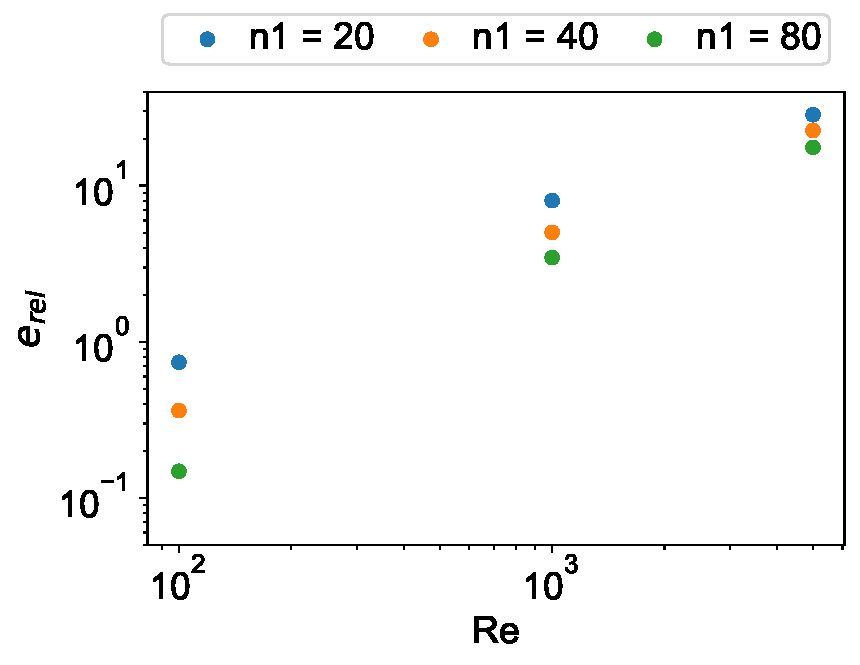
\includegraphics[width=\textwidth]{termino_adv_UP1.pdf}
      \caption{}
      \label{fig:termino_adv_UP1}
  \end{subfigure}
  \hfill
  \begin{subfigure}[b]{0.32\textwidth}
      \centering
      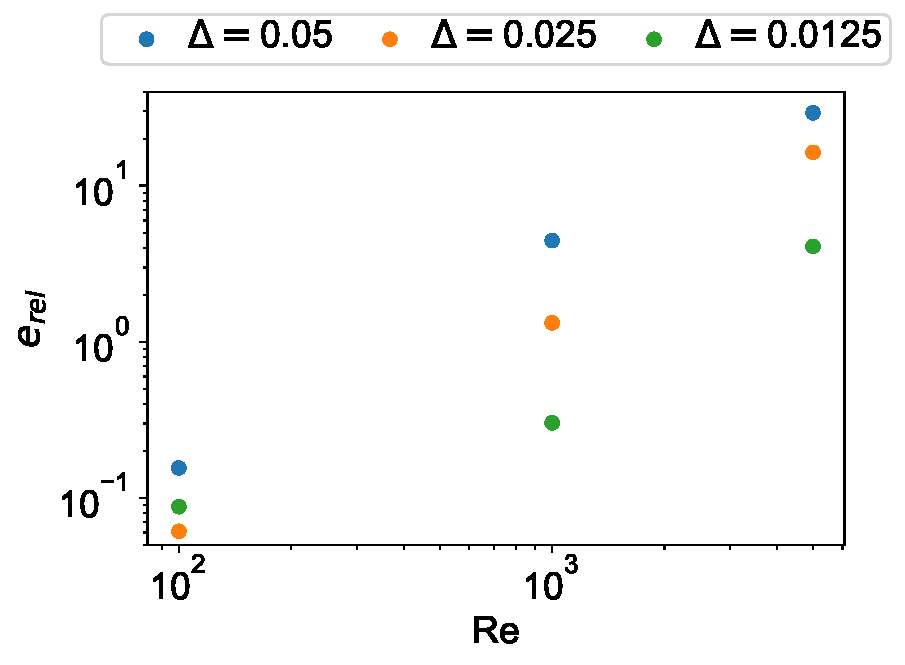
\includegraphics[width=\textwidth]{termino_adv_QUICK.pdf}
      \caption{}
      \label{fig:termino_adv_QUICK}
  \end{subfigure}
     \caption{Termino advectivo \textcolor{red}{Ponerle a los 3 los mismos ejes}}
     \label{fig:termino_advectivo}
\end{figure}



\twocolumngrid




\begin{table}[]
  \begin{tabular}{l|ccc|}
  \cline{2-4}
                            & \multicolumn{3}{c|}{$e$}                                                    \\ \hline
  \multicolumn{1}{|l|}{DC2} & \multicolumn{1}{c|}{$0.08541$} & \multicolumn{1}{c|}{$0.17567$} & $0.69045$ \\ \hline
  \multicolumn{1}{|l|}{UP1} & \multicolumn{1}{c|}{$0.14813$} & \multicolumn{1}{c|}{$3.46833$} & $17.6402$ \\ \hline
  \multicolumn{1}{|l|}{QUICK} & \multicolumn{1}{c|}{$0.08778$} & \multicolumn{1}{c|}{$0.30266$} & $4.09139$ \\ \hline
  \end{tabular}
  \end{table}

\textcolor{blue}{Tabla con resultados}



\textcolor{red}{Duda: es necesario reportar el dt en cada caso? No lo voy a hacer}














\subsection{Orden de convergencia espacial de UP1}

Se calculó $u(0.5)$ y $v(0.5)$ para $Re = 1$ y $Re = 1000$ con $n1 = 80$ y esquema QUICK. Se consideró este valor como la solución exacta. Luego, se calcularon las mismas velocidades para distintos n1 y se calculó el error respecto a la solución numérica considerada como la exacta

\begin{figure}[h]
  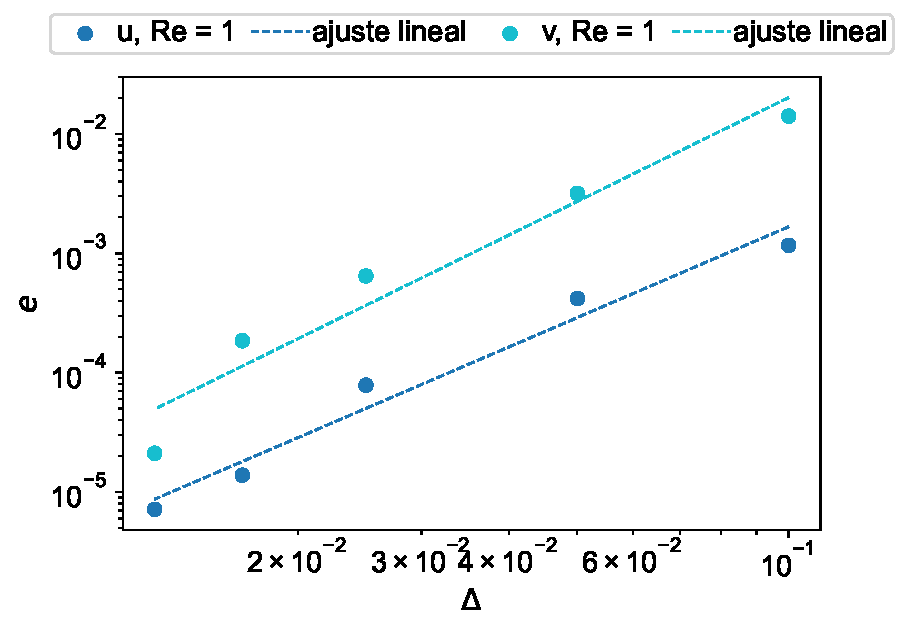
\includegraphics[clip=true,width=\columnwidth]{error_UP1_n1_vs_Re.pdf}
  \caption{}
   \label{fig:error_UP1_n1_vs_Re}
\end{figure}

u: Orden de convergencia:  2.5279722490866563 +/- 0.25890392418605823
v: Orden de convergencia:  2.88403428611868 +/- 0.4040887289633906


\subsection{Esquema temporal con solución dependiente del tiempo}


\textcolor{blue}{Evolución temporal con EI y CN.}





\section{Conclusión}

\bibliography{Chehade_final.bib}

\end{document}





